\section{Corpus construction and scoring}\label{app:corpus}

Section~\ref{sec:method} states the corpus and the reading in four paragraphs. This appendix gives what the body leaves out: the selection rule and the two filters, the systems that pass the two-loop audit, the promotion scopes, the substrate rubric with its distribution over the corpus, and the evidence rules behind every classification.

\subsection{What is read for each system}\label{what-is-read-for-each-system}

We read each system's public method or documentation for four things: the persistent artifact it changes, the feedback that prompts the change, the decision that accepts it, and the scope in which the result is used. This allows systems with different names and application domains to be compared by their behavior.

\subsection{Scope and selection}\label{scope-and-selection}

The corpus contains 256 unique systems from January 2023 through the October 2026 cutoff. The first search pass identified 130 systems by May 2026; the second added 126. Sources include research papers, public repositories, product documentation, and supported production reports; the search families, evidence tiers, and inclusion rules are recorded with the released data in the supplementary material.

A system enters the survey if it adapts a foundation model through a persistent artifact updated from deployment signal, or if it is publicly described as self-improving, scaffolded, or agentic. Including the latter group provides a contrast set: the survey can test whether those descriptions correspond to persistent adaptation. Systems whose only update mechanism is weight-level training are excluded, as are systems without public evidence of release or deployment.

We apply two filters. The first admits a system to the \textbf{core corpus} if it scores at least 3 on at least one scaffold substrate under the rubric below. Of the 256 systems, 204 form the core corpus and 52 the contrast corpus. A system may have one integrated row or several substrate-specific rows, so the 256 systems occupy 269 scored rows.

The second filter is a \textbf{two-loop audit}. It asks whether session feedback changes a persistent artifact and whether that artifact is subsequently promoted beyond the deployment that produced it, with versioning or lineage. Applied to 202 of the 204 core systems and to 4 research systems classified from their papers alone (SkillOpt, FederatedSkill, SkillClaw, and ChronoMem), it admits 11 research systems and 3 industry exemplars; two core systems (COSPLAY and Cuadros et al.) and six paper-classified ones (PACE, CORAL, GEPA, Meta-Harness, MOSS, and RCL) carry no audit. Fig.~\ref{fig:corpus} summarizes the selection.

\begin{figure}[h]
\centering
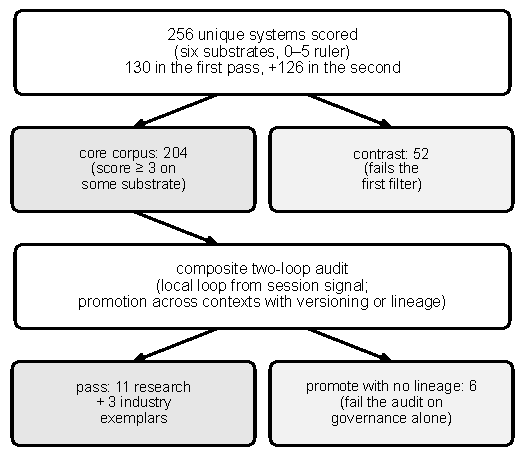
\includegraphics[width=\columnwidth]{figures/fig4_corpus_flow}
\caption{Corpus selection. The 256 systems occupy 269 scored rows. The first filter separates core from contrast systems; the two-loop audit then checks persistent local adaptation and promotion with lineage. The audit includes the additional paper-based classifications described in the text.}
\label{fig:corpus}
\end{figure}

The research systems passing the audit are NanoResearch, SkillOpt, AlphaEvolve, ADAS, DGM, Voyager, SAGE, EvolveR, CoEvoSkills, AutoManual, and CASCADE. The industry exemplars are Sierra Agent OS 2.0, Cognition Devin, and Letta's Context Repositories. SkillOpt is classified from its paper and is not a row in the 256-system score table. The remaining paper-based systems are identified in the data notes, and the audit's boundary cases in the contrast set, both in the supplementary material.

Passing this audit does not establish governed sharing across organizations. All passing systems promote within one operator, into a shared bank or archive that later runs draw from, or across the agents and sessions of one deployment. Letta passes on the lineage of its shared-memory updates even though those updates have no acceptance gate. Six further systems promote across contexts without lineage on the promoted artifact; their treatment under relaxed audit rules is reported in Appendix~\ref{app:grid}.

\subsection{Promotion scopes}\label{promotion-scopes}

The scope in which an accepted edit is used is read on five nested levels. \textbf{USER} covers one person's account or fork. \textbf{PROJECT} covers a repository, workflow, or product workspace. \textbf{STACK} is a team's curated bundle of projects. A \textbf{TENANT} is an organization or customer, and \textbf{CORE} is the scope shared by all tenants. A wider scope aggregates the losses of the deployments it contains. Promotion changes which population the edit is intended to improve, as shown in Fig.~\ref{fig:scope}; Appendix~\ref{app:governed} takes up what a check at the receiving scope can and cannot establish.

\begin{figure}[h]
\centering
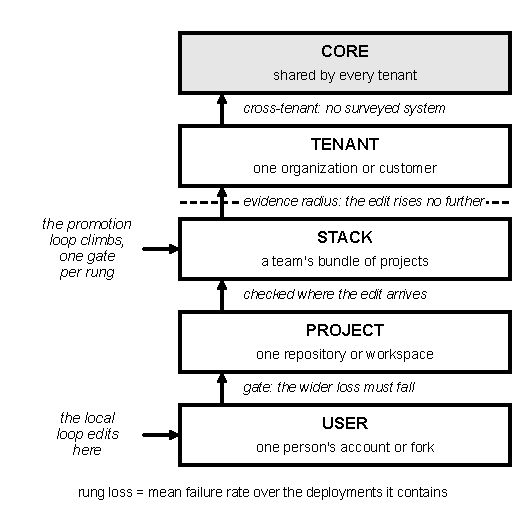
\includegraphics[width=\columnwidth]{figures/fig2_scope}
\caption{Promotion scopes, from a user account to the shared core. Wider adoption changes the population on which an edit acts. Receiving-side evaluation checks whether the improvement is supported for the recipient.}
\label{fig:scope}
\end{figure}

\subsection{Substrates and scoring}\label{substrates-and-scoring}

The scaffold has six substrates: instructions, skills, memory, tools, orchestration, and governance. These are the possible targets of a proposed edit. Table~\ref{tab:substrates} describes them; the episodic, semantic, and procedural memory categories follow \citet{sumers2023coala}.

\begin{table*}[h]
\centering\small
\begin{tabular}{>{\raggedright\arraybackslash}p{0.17\textwidth}>{\raggedright\arraybackslash}p{0.38\textwidth}>{\raggedright\arraybackslash}p{0.40\textwidth}}
\toprule
Substrate & What persists & A score of 5 requires \\
\midrule
S1 Instructions & Project, team, or organization rules attached to a workspace & Versioned rules promoted under an automatic gate \\
S2 Skills & Procedures, as code or text, loaded on demand & A skill bank that edits itself on failure, test-gated, versioned, and promoted \\
S3 Memory & Experience kept across sessions: episodic, semantic, procedural & Provenance, versions, and a correction path for every entry \\
S4 Tools & The vetted action surface and its schemas & Evaluation-gated tool versions; a curated bundle as the product \\
S5 Orchestration & The multi-role graph and its routing & Topology updated from deployment feedback by a loop outside the agent's own run \\
S6 Governance & Versioning, promotion, audit, rollback & Staged promotion with evaluation thresholds, an audit log, and rollback \\
\bottomrule
\end{tabular}
\caption{The six scaffold substrates, what each holds, and what a system must do on it to score 5.}
\label{tab:substrates}
\end{table*}

The common scoring scale runs from 0 to 5. At 0 an artifact is ephemeral. At 1 it persists locally; at 2 it persists with tool attachment but without feedback. At 3 it either spans scopes without a gate or is updated from feedback by a person. At 4 a program updates it from feedback. The score-5 requirement depends on the substrate, as specified in the table.

This last distinction is important when interpreting the scores. Instructions and skills require both loops to reach 5. Orchestration requires a topology updated from deployment feedback by a loop outside the agent's own execution. Memory, tools, and governance are scored for their corresponding governance capabilities, so a registry can score 5 without generating local edits. Integrated rows measure breadth and depth of adaptation, not closure of either loop. The scale therefore supports substrate-specific comparisons; a top score is not a universal certificate of complete optimization.

Table~\ref{tab:maturity} gives the corpus distribution. Research systems hold the top marks on skills, memory, and the integrated row, and production platforms hold them on governance. No system reaches the top score across all six substrates, and none reaches it on instructions, tools, or orchestration.

\begin{table*}[h]
\centering\small
\begin{tabular}{>{\raggedright\arraybackslash}p{0.13\textwidth}>{\raggedright\arraybackslash}p{0.04\textwidth}>{\raggedright\arraybackslash}p{0.05\textwidth}>{\raggedright\arraybackslash}p{0.25\textwidth}>{\raggedright\arraybackslash}p{0.48\textwidth}}
\toprule
Substrate & $n$ & Mean & Score-5 systems & What the corpus holds on it \\
\midrule
S1 Instructions & 15 & 3.07 & (none) & Rules persist across IDEs and agents and nothing measures them; no system closes both loops; ceiling 4 \\
S2 Skills & 50 & 3.34 & SAGE, COSPLAY & The local loop closes under a program in the research systems; the production repositories merge by hand \\
S3 Memory & 50 & 3.06 & Cuadros et al. & The ledger ships in products; the correction a gate would enforce is absent \\
S4 Tools & 20 & 3.35 & (none) & Production tools are widely shared; registries govern admission, not evaluation \\
S5 Orchestration & 37 & 3.08 & (none) & Topologies change under an evaluation gate; one structurally gated instance; no two-loop system with lineage \\
S6 Governance & 45 & 2.98 & Braintrust, Vellum, LangSmith Hub & Prompts-as-code mature; registries add lineage and rollback; no local loop generates a candidate \\
Integrated & 52 & 3.81 & NanoResearch, AutoAgent, SkillRL & Breadth and depth of adaptation, not the loop; reached only by research systems without enterprise governance \\
\bottomrule
\end{tabular}
\caption{Substrate maturity across the 256-system corpus. Column $n$ counts scored rows on each substrate, Mean is the average score, and Score-5 systems reach the substrate's top mark; the integrated row counts systems scored across several substrates as one row. Of the 126 most recently added systems, 105 are core and 32 are skill systems; 96 of those core systems have a local loop and 89 close it under a program, and none of the 126 scores 5 on any substrate.}
\label{tab:maturity}
\end{table*}

For the 126 most recently added systems, gate types, feedback classes, and governance properties are recorded as explicit columns of the released table, so counts based on those columns apply to those systems. For example, 96 of their 105 core systems have a local loop, and 89 of those close it under a program. This is not a gate count over all 256 systems.

\subsection{Instruction files}\label{instruction-files}

The instructions substrate never reaches the top score, yet it holds the most widely deployed artifact. Instruction files are present across Claude Code, Cursor, AGENTS.md \citep{agentsmd2025}, Windsurf, and Continue.dev, and adoption studies find them in roughly a fifth to a quarter of coding-agent projects \citep{robbes2026agenticmuch, galster2026harnessconfig}. Their prevalence does not settle their effectiveness. One controlled study reports higher inference cost without improved task success \citep{gloaguen2026agentsmd}. Another toggles the root AGENTS.md in paired runs on 124 pull requests and reports about 29\% lower median wall-clock time and 17\% fewer median output tokens, with total tokens approximately unchanged; it does not measure correctness \citep{lulla2026empirical}. The studies measure different outcomes and disagree on cost. Neither establishes a general task-success benefit from accumulating instruction files.

\subsection{Evidence and limitations}\label{evidence-and-limitations}

The evidence ranges from peer-reviewed studies and open-source artifacts to vendor claims. Every row of the released table carries its source and a one-line justification, and the rows for the 126 most recently added systems also carry an evidence tier. Peer-reviewed papers and open-source artifacts receive the greatest weight. A production claim must name a benchmark or integration target, and a blog or interview is counted only when stronger evidence corroborates it. Production claims are not pooled with peer-reviewed evidence in corpus-level statistics; vendor-based exemplars are identified as such.

One author scored all systems. Ambiguous cases were rounded down, and half-scores were used only when one criterion was clearly met and another partly met. Independent re-rating remains future work. The classifications should be read as an auditable interpretation of public evidence, not a complete inventory of private production behavior.

We also test the audit under alternative boundaries: counting rollback as sufficient promotion governance, allowing promotion without governance, and admitting loops that persist only optimizer state. Membership changes under these relaxations, but the principal structural findings remain: {[}Auto \(\times\) Auto{]} stays well populated, the human-local cells hold only curation and registries, Letta alone passes with an ungated promotion, and no relaxation adds governed promotion across organizations (Appendix~\ref{app:governed}). The sensitivity analysis is released with the data notes and the full score table with the released table, both in the supplementary material.

\section{Formal statement of the loop}\label{app:formal}

Section~\ref{sec:loop} states the local loop in words and its acceptance rule in one line. This appendix carries the mathematics behind it: the patch loss and the gate, the update rule, a one-step descent inequality under a noisy gate, an informal convergence proposition, the optimization-analogy correspondence, four worked cases, and SkillOpt as a published instance of all five conditions. No new theorem is claimed; the proposition is the ordinary target of local stochastic optimization under noisy estimators, restated for a discrete, versioned parameter.

\subsection{Patch loss and the acceptance rule}\label{patch-loss-and-the-acceptance-rule}

For deployment \(D\), write the patch loss as \[L_D(\theta_s)=\mathbb{E}_{x\sim D}\!\left[\ell(\pi(\theta_M,\theta_s,x))\right],\] where \(\theta_M\) denotes the fixed model weights, \(\theta_s\) the editable scaffold, and \(\ell\) the operational loss. A proposal process uses the failure history to produce an edit \(z_t\). There is no analytic gradient through an instruction file or memory entry. Instead, the gate estimates the change in loss and accepts when that estimate clears a required margin: \[G_t(z_t)=1\iff\widehat{\Delta}_{z_t}L_D(\theta_s^t)+\lambda\Omega(z_t)\leq-\tau_t.\] Here \(\Omega\geq0\) penalizes edit complexity and promotion breadth, and \(\tau_t\geq0\) is the acceptance margin. An evaluation that blocks a regressing merge is a practical instance of this rule. A reviewer or governance process can also instantiate the gate by requiring stronger evidence for a broader or more complex change.

\subsection{Setup}\label{setup}

Let the frontier model have fixed parameters \(\theta_M\) and let the scaffold be a structured object \(\theta_s \in \Theta_s = \Theta_1 \times \cdots \times \Theta_6\) over the six substrate coordinates of Appendix~\ref{app:corpus}; \(\Theta_s\) is discrete, symbolic, and versioned. For a deployment \(D\), \(L_D(\theta_s) = \mathbb{E}_{x \sim D}[\ell(\pi(\theta_M, \theta_s, x))]\). A candidate edit \(z_t \sim Q_t(z \mid H_t, \theta_s^t)\) is drawn from a proposal process conditioned on the accumulated history \(H_t\) of failures, corrections, rejected outputs, evaluation regressions, and prior accepted edits. \(Q_t\) is not uniform: for a mode \(m\) that recurs with frequency \(f_m\) and carries per-occurrence loss \(s_m\), its expected contribution to the failure rate is \(f_m s_m\), so high-frequency or high-severity modes are proposed first. The finite directional difference is \(\Delta_z L_D(\theta_s) = L_D(\theta_s \oplus z) - L_D(\theta_s)\); the gate sees only a noisy estimate \(\widehat{\Delta}_z L_D\). The update is \[\theta_s^{t+1} = \theta_s^t \oplus z_t \text{ if } G_t(z_t) = 1, \quad \theta_s^{t+1} = \theta_s^t \text{ otherwise.}\]

\subsection{Descent inequality}\label{descent-inequality}

Write \(\mathcal{F}_t\) for the history up to step \(t\): the failures, corrections, edits, and gate decisions in \(H_t\) together with \(\theta_s^t\). Because the proposal \(Q_t\) depends on the whole history and not on \(\theta_s^t\) alone, every expectation and probability below conditions on \(\mathcal{F}_t\). Assume (A1) positive descent bias on accepted edits, \(\mathbb{E}[\widehat{\Delta}_{z_t} L_D \mid G_t = 1, \mathcal{F}_t] \le -\gamma_t - \tau_t\) for some \(\gamma_t > 0\), and (A2) bounded estimator bias on accepted edits, \(|\mathbb{E}[\Delta_{z_t} L_D - \widehat{\Delta}_{z_t} L_D \mid G_t = 1, \mathcal{F}_t]| \le \varepsilon_t\). With \(p_t = \Pr(G_t = 1 \mid \mathcal{F}_t)\), \[\mathbb{E}[L_D(\theta_s^{t+1}) \mid \mathcal{F}_t] \le L_D(\theta_s^t) - p_t(\gamma_t + \tau_t) + p_t\,\varepsilon_t.\] Per-step expected improvement is the gate's margin minus its estimator bias, weighted by acceptance probability. In the feedback-signal classes of Section~\ref{sec:signal}, \(\varepsilon_t\) is near zero for the check itself in C1, with the sampling error of a finite suite over the patch remaining, bounded by batching for an observable outcome (C2), equal to the judge's bias and bounded only by calibration for a judged signal (C3), and unavailable per edit for a delayed signal (C4).

\subsection{Convergence (informal)}\label{convergence-informal}

What follows is a conditional statement under strong assumptions, included to make gate stability precise; nothing in the survey depends on it. Add (A3) proposal coverage with acceptance: at every non-gate-stable scaffold, \(Q_t\) places probability at least \(q > 0\) on an admissible edit with \(\mathbb{E}[\Delta_z L_D] \le -\delta\), and the gate accepts such an edit with probability at least \(q' > 0\), so that \(p_t(\gamma_t + \tau_t) \ge q q' \delta\) there; (A4) effective compactness of the reachable orbit; and (A5) summable bias, \(\sum_t p_t \varepsilon_t < \infty\); and let \(0 \le L_D \le B\). (A3) is strong: it asks for a uniform lower bound on proposing and accepting an edit that lowers the loss by at least \(\delta\), which needs attribution far more reliable than success with non-zero probability per failure. The one-step inequality is then of the Robbins--Siegmund form, a non-negative process that decreases in expectation up to a summable perturbation \(p_t \varepsilon_t\), so \(L_D(\theta_s^t)\) converges almost surely and \(\sum_t p_t(\gamma_t + \tau_t) < \infty\) almost surely \citep{robbins1971convergence}. The finite sum carries the content: a bounded loss cannot pay for infinitely many accepted edits with a positive expected margin, so under (A3) the process visits non-gate-stable scaffolds only finitely often, and with (A4) the limit set of \(\{\theta_s^t\}\) is gate-stable: no admissible edit clears the gate with negative expected directional loss in the limit. This is convergence of the loss and stability of the gate decision, not convergence to an optimum; a globally suboptimal gate-stable scaffold is consistent with the result, because \(Q_t\) may never propose the improving edit or \(\widehat{\Delta}\) may be biased to reject it. A non-stationary deployment (\(D = D_t\)) falls outside this argument: tracking a moving optimum would need further assumptions on the rate of drift and of adaptation, which are not supplied here. Recency weighting, pruning, expiry, and rollback are the scaffold-level analogues of the machinery continual learning uses for that case.

\subsection{Correspondence}\label{correspondence}

Table~\ref{tab:optim} pairs each optimization concept with its scaffold analogue. Credit assignment here is attribution, not backpropagation. Scaffold systems do not differentiate through instruction files. They trace an output error to an upstream coordinate, manually or with a judge or verifier. The one-step inequality needs only that accepted edits have positive expected descent; the convergence statement needs attribution reliable enough to supply the uniformly improving proposals that (A3) assumes, which is much stronger than the credit-assignment condition of Section~\ref{sec:loop}, success with non-zero probability per failure.

\begin{table*}[h]
\centering\small
\begin{tabular}{>{\raggedright\arraybackslash}p{0.25\textwidth}>{\raggedright\arraybackslash}p{0.70\textwidth}}
\toprule
Optimization concept & Scaffold analogue \\
\midrule
Parameter vector & Instructions, skills, memories, tools, routing graphs, and governance rules, evaluation gates among them \\
Loss & Failure, user correction, evaluation regression, retrieval miss, tool error, schema violation \\
Gradient estimate & Credit assignment identifying the coordinate responsible for a failure \\
Step & Accepted scaffold edit; step size is edit magnitude under $\oplus$ \\
Aggregated update & Several recurring failures combined before an update, by averaging or by agreement across $k$ proposals \\
Update radius & Promotion scope: which loss is descended (USER, PROJECT, STACK, TENANT, CORE) \\
Validation loss & Held-out patch evaluation before merge \\
Regularization & Complexity penalty $\Omega(z)$, bloat control, cross-patch regression checks \\
Overfitting & Scaffold improves on this deployment and degrades elsewhere \\
Rollback & Reverting a harmful accepted update \\
\bottomrule
\end{tabular}
\caption{Optimization concepts and their scaffold analogues.}
\label{tab:optim}
\end{table*}

\subsection{Worked cases}\label{worked-cases}

\emph{Retrieval.} Failures recur because retrieved context omits the decisive clause. Attribution traces the error to the retrieval coordinate: chunking, query rewriting, metadata filter, embedding model, reranker, or context-packing rule. The candidate edit tightens chunk boundaries or adds a metadata constraint, and the gate checks that recall and answer accuracy improve on the patch evaluation without degrading adjacent cases. Signal class C1 or C2.

\emph{Pitch review.} The system repeatedly overrates decks that claim a large market without numbers, and the failure cluster points at an under-specified rubric coordinate. The edit changes ``evaluate market size'' into ``require a numeric estimate and a source; if absent, cap the score''; the gate runs the revised rubric against held-out decks with human scores. What the edit changed was the gate that will judge the next edit: the reflexive gate of Section~\ref{sec:evaluator}, class C3.

\emph{Tool use.} Calls fail because optional parameters are under-specified. The responsible coordinate may be the tool schema, the call policy, or the clarification rule. The edit adds required fields or a pre-call uncertainty check; the gate checks that tool-call failures fall without raising refusals or latency. Class C2.

\emph{Memory.} A stale customer preference is repeatedly retrieved and causes bad decisions. The responsible coordinate is a memory entry together with its provenance, priority, and expiry policy. The edit corrects, expires, or version-tags the entry; the gate checks that future behavior improves without erasing useful history. Class C2, with the correction itself observable only when a later outcome reveals it.

\subsection{A complete local example}\label{a-complete-local-example}

SkillOpt provides a concrete instance of all five conditions \citep{yang2026skillopt}. Its persistent state is one markdown skill document used by a frozen agent. Rollout and reflection batches supply the failure evidence. A consensus filter helps attribute recurring errors, and bounded add, delete, and replace operations propose changes. A held-out exact-match split supplies the loss, and a candidate is accepted only when its score strictly improves.

Across six benchmarks, seven target models, and three harnesses, SkillOpt is best or tied in every cell reported by its authors. Its follow-up, SkillOpt-Lite, removes a rejected-edit buffer and slow update schedule while retaining the held-out gate and consensus filter; it matches or exceeds the original \citep{shen2026skilloptlite}. This comparison supports the importance of the gate and this form of credit assignment in that setting, while identifying the removed controls as stabilizers rather than necessities.

SkillOpt also evaluates transfer across models, harnesses, and benchmarks. Those experiments measure how far the learned artifact remains useful. They are distinct from the acceptance decision that admits an edit to the shared skill bank.

\section{Gate families and feedback classes}\label{app:gates}

Section~\ref{sec:signal} gives the four feedback classes with one developed example each (Table~\ref{tab:classes}), and Section~\ref{sec:local} states the difference between agreement and averaging in one sentence. This appendix lists the gate families that instantiate the acceptance test and the class each serves, sets out the batching distinction, and develops each class with the systems that fall in it.

\subsection{Gate families}\label{gate-families}

Section~\ref{sec:loop} collapses every production gate into one per-edit test \(G_t\) on an estimate of the loss change. Surveyed systems instantiate that test in several distinct ways, and some of them are better read as proposal pruning that precedes the per-edit gate than as estimators of \(\widehat{\Delta} L_D\). Table~\ref{tab:gatefamilies} lists the families, the slot each occupies, representative systems, and the feedback-signal class each family serves.

\begin{table*}[h]
\centering\small
\begin{tabular}{>{\raggedright\arraybackslash}p{0.12\textwidth}>{\raggedright\arraybackslash}p{0.20\textwidth}>{\raggedright\arraybackslash}p{0.13\textwidth}>{\raggedright\arraybackslash}p{0.17\textwidth}>{\raggedright\arraybackslash}p{0.33\textwidth}}
\toprule
Gate family & What it estimates & Slot in Section~\ref{sec:loop} & Signal class & Representative systems \\
\midrule
Surrogate verifier & Pass or fail from tests, a symbolic checker, or an exact match & Per-edit gate $G_t$ & C1 & DGM (sandboxed compile-and-edit check; score weights selection, not retention), SkillOpt (held-out exact match), Voyager (game-state check: C2) \\
Evaluation cascade & $\widehat{\Delta} L_D$ on a held-out task suite, cheap-to-expensive evaluators & Per-edit gate $G_t$ & C1 when the suite is exact; C2 when it is a task suite & AlphaEvolve, Braintrust, Vellum, LangSmith Hub \\
RL threshold & Reward improvement against a deployment threshold & Per-edit gate $G_t$ & C2 & SAGE, PACE \\
LLM judge with calibration & Pairwise or rubric score, calibrated against human agreement & Per-edit gate $G_t$ & C3 & SkillChain (judge stage, before its human reflection gate) \\
Reviewer judgment & Human credit assignment by pull-request review, expert sign-off, or a user's acceptance & Per-edit gate $G_t$, human-instantiated & C3 (and C2 when the reviewer has outcome data) & Sierra Agent OS 2.0, Anthropic skills repository, CASCADE (a person and an agent approve consolidation into shared memory) \\
Semantic merge & Whether a candidate duplicates or conflicts with existing artifacts & Proposal pruning before $G_t$ & C4 (also a pre-filter in C2, C3) & NanoResearch orchestrator, FederatedSkill server agent, EvolveR (admission: cosine pre-filter plus LLM equivalence judgment on each distilled principle; retention: periodic pruning on per-principle success rate) \\
Archive selection & Whether a candidate improves on, or diversifies, an archive of already-scored programs & Proposal pruning before $G_t$ & Any; inherits the class of the evaluator that scored the archive (C1 in AlphaEvolve) & AlphaEvolve (MAP-Elites-style database), ADAS \\
Multi-sample agreement & Whether $k$ independent proposals or evaluations agree; false-accept rate decays as $p^k$ rather than variance as $1/k$ & Aggregation filter on the estimate & C2, C3 noise absorption & VaG (three heterogeneous critics must all pass); SkillOpt-Lite (consensus filter across rollouts) \\
\bottomrule
\end{tabular}
\caption{Gate families, their slot in the formalism, and the feedback-signal class each serves.}
\label{tab:gatefamilies}
\end{table*}

The first five families populate \(G_t\) directly and, under the assumptions of Appendix~\ref{app:formal}, inherit its descent guarantee. Semantic merge and archive selection are not estimators of \(\widehat{\Delta} L_D\); they constrain the proposal distribution, and the descent argument applies to the composition of pruning and gate. Multi-sample agreement is listed because it is the correct analogue of ``wait for \(k\) pieces of evidence before accepting an edit'', a different operation from mini-batch averaging and one that should not be conflated with it. Read down the signal-class column. The only families available to a judged (C3) deployment are the two whose estimator is a judge. A delayed (C4) deployment has no family that estimates the loss change per edit at all: what it has is semantic merge before the gate and whatever proxy milestone stands at the horizon. That is the structural content of Section~\ref{sec:signal}.

\subsection{Agreement and averaging}\label{agreement-and-averaging}

An acceptance test can itself be too noisy to support a decision from one run. Several newer systems address this directly. SAGE-gate, a statistical acceptance method unrelated to SAGE, uses paired per-item comparisons before committing an edit \citep{wang2026sagegate}. VaG requires three heterogeneous critics to pass \citep{shang2026vag}. AutoSaddler uses mini-batch failure signals in validation-based selection \citep{park2026autosaddler}.

These mechanisms should not be conflated. Averaging \(k\) independent noisy scores reduces the variance of their mean by a factor of \(1/k\). Requiring agreement among \(k\) independent checks, each with false-acceptance probability \(p\), gives the idealized probability \(p^k\). The independence assumptions matter, and actual critics need not satisfy them. The shared development is that acceptance increasingly depends on a body of evidence rather than one favorable observation.

\subsection{Assigning a class}\label{assigning-a-class}

The classes are assigned by the constraint that binds first. A long delay makes a signal C4 even when the eventual outcome is objective. Among timely signals, the absence of an independent ground truth makes the signal C3. Among timely objective signals, repeatable exact checks distinguish C1 from noisy observed outcomes in C2. A system may use several signals, but its operative acceptance decision must be read against the signal that supports it.

\subsection{Exact checks (C1)}\label{exact-checks-c1}

A compiler, proof checker, schema validator, or exact-match answer key can decide a specified property immediately and repeatably. This makes an automatic gate straightforward to implement. AlphaEvolve scores candidates through a cascade of exact evaluators \citep{alphaevolve2025}, and SkillOpt uses held-out exact-match evaluation \citep{yang2026skillopt}. DGM makes a narrower acceptance decision: it retains self-modifications that pass a sandboxed compile-and-edit functionality check on ten benchmark tasks. The broader benchmark score weights parent selection from the archive rather than determining retention \citep{zhang2025darwin}.

Exactness applies to the check, not to the deployment as a whole. Repeating a deterministic check on the same output yields the same answer, but an agent produces stochastic outputs, and a finite suite samples only part of the task distribution. Estimating the change in patch loss still requires accounting for that variation. Passing the suite also establishes only the properties the suite tests.

Two problems remain even with a reliable checker. A failed test may not identify the instruction or skill that caused the failure, and repeated optimization against the same suite can overfit it. Cheap acceptance can also allow the artifact pool to grow without sufficient pruning. Exact feedback makes evaluation easier; it does not supply attribution or lifecycle management.

\subsection{Observed outcomes (C2)}\label{observed-outcomes-c2}

A booked appointment, closed ticket, merged pull request, or successful tool call provides an observable result after an episode. The result is meaningful but may be noisy or confounded. A user can accept an incorrect answer or reject a correct one, and a merged pull request reflects more than the agent's technical performance.

Devin reads merged pull requests as feedback \citep{cognition2025devinreview}. SAGE measures task success in AppWorld \citep{wang2025sage}, and PACE uses failure signals from a deployed small model \citep{ling2026pace}. SkillRL uses a success-rate threshold only to trigger proposals, without testing whether the proposed skills should remain \citep{skillrl2026}. The same kind of outcome can therefore support different operations in different systems.

Simulated outcomes, such as those in Voyager's game world or SAGE's AppWorld, remove the user confound and can be sampled repeatedly. They are treated as a distinguishable case within C2. For observed outcomes more generally, an automatic gate needs a positive margin and enough episodes or independent evidence to absorb noise. Even then, the result usually reveals that the task failed more readily than why it failed.

Promotion is harder because another deployment may differ in users, tasks, and acceptance behavior. A sender's successful outcome is not an evaluation of the recipient. This class also depends on channels that can carry poisoned memories or injected tool instructions, connecting the reliability of feedback to the integrity of its source.

\subsection{Judgments (C3)}\label{judgments-c3}

For style, persuasion, design, or other preference-dependent tasks, a gate relies on a person, rubric, reference comparison, or model judge. There is no independent exact answer to the preference being measured. CASCADE uses a human-and-agent gate for memory consolidation \citep{huang2025cascade}, and a reviewer approves promotion into Anthropic's skills repository. SkillForge uses its calibrated judge earlier in the process, to identify replies that motivate a rewrite \citep{skillforge2026}.

A program can make these decisions, but its score must be calibrated against the human judgment it is intended to represent before the score is treated as evidence of that preference. The gate labels deliberately do not record this distinction: an uncalibrated model judge is still an Auto gate, though the meaning of its acceptances is less established. SkillForge, SkillChain, and SkillCoach report calibration measurements \citep{skillforge2026, hu2026skillchain, zhu2026skillcoach}; no other surveyed judge does.

Optimization introduces another risk. A scaffold can become better at satisfying the judge while becoming worse at the underlying task. Reward-model research measures this form of proxy overoptimization \citep{gao2023overoptimization}. Human evaluation is not fixed either: \citet{shankar2024validators} find that evaluators' criteria change as they grade more outputs. If the system also edits the rubric, it changes the instrument used to assess subsequent edits. This \textbf{reflexive gate} is developed in Section~\ref{sec:evaluator} and, with the weight-side comparison, in Appendix~\ref{app:failure}.

\subsection{Delayed and sparse outcomes (C4)}\label{delayed-and-sparse-outcomes-c4}

Research programs and open-ended discovery may produce meaningful outcomes only after weeks or months and many intervening edits. The AI Scientist illustrates the broad setting by generating ideas, conducting experiments, and writing a paper \citep{lu2024aiscientist}. The eventual outcome cannot usually be assigned to each preceding scaffold change.

Systems in this class consequently use intermediate decisions. NanoResearch merges skills by semantic compatibility \citep{xu2026nanoresearch}. CORAL promotes findings into shared memory on a heartbeat \citep{qu2026coral}. These operations can prune or consolidate proposals, but they do not estimate each edit's contribution to the eventual loss. AlphaEvolve's archive diversity does not make it a delayed-signal example: its candidates have already been scored by exact evaluators, so archive selection is a search strategy within C1 \citep{alphaevolve2025}.

For C4, the descent interpretation applies only to whatever proxy gate is available or to an evaluation at the longer horizon. Temporal credit assignment remains unresolved, and the environment can change before the result arrives. Outcome gains alone are also insufficient to distinguish directed improvement from a successful search, a limitation emphasized in the evaluation of harness optimizers \citep{ong2026harnesseval}.

\section{The gate grid in detail}\label{app:grid}

Section~\ref{sec:promotion} reads the gate grid of Fig.~\ref{fig:grid} in one paragraph, and Section~\ref{sec:signal} states the three expectations the grid tests. This appendix gives the systems behind each local-gate and promotion-gate value, the infrastructure that fills the bottom row, the grid cell by cell with its boundary cases, and how the expectations fare against the corpus.

\subsection{Who keeps a local edit}\label{who-keeps-a-local-edit}

Research systems commonly generate candidates by reflecting on trajectories. In production prompt platforms, an engineer writes the candidate and session feedback never triggers one, while public skill repositories depend on contributors. A field study of five such repositories finds that every substantive edit was committed under a named human account and merged by a person, most carrying an AI co-author trailer \citep{shen2026whomaintains}. Where proposal generation depends on a person noticing a problem, the evaluation machinery can run automatically while the improvement process itself remains intermittent.

On skills, SAGE and COSPLAY close both local and promotion loops inside a research environment \citep{wang2025sage, wu2026cosplay}. SkillChain adds a human reflection decision after the judge, on which refined skills are deployed \citep{hu2026skillchain}. SkillRL and SkillForge leave the proposed changes unchecked. These differences would be obscured by classifying all three simply as systems that learn from feedback.

Orchestration has followed a similar progression. Early systems searched for agent topologies under an evaluation score \citep{zhuge2024gptswarm, zhang2024aflow}. More recent systems evaluate proposed topology changes before keeping them; TOCOMAS also requires a structural invariant \citep{chu2026agentgrad, chen2026harnessforge, zhao2026tocomas}. OptiMAS is an exception: its optimizer reads trajectories and validation scores to write the next configuration, but the score informs the edit rather than supplying a keep-if-better decision \citep{cheng2026optimas}. No orchestration system closes both loops with lineage on the promoted artifact.

Human local gates appear only in curation. VerificAgent uses fact-checked, frozen memories \citep{nguyen2025verificagent}, and in SkillChain a person decides, at a reflection gate, which refined skills are deployed. Prompt platforms and registries without a failure-driven proposal process have no local gate in this classification. Their checks act on release or admission to a shared pool, which belongs to promotion.

\subsection{Who lets an edit climb}\label{who-lets-an-edit-climb}

Research systems often promote by admitting a candidate to a bank or archive that later runs reuse. SkillOpt, DGM, ADAS, Voyager, and SAGE apply programmatic decisions within this shared environment \citep{yang2026skillopt, zhang2025darwin, hu2024adas, wang2023voyager, wang2025sage}. AlphaEvolve and its predecessor FunSearch score candidates before archive admission \citep{alphaevolve2025, romeraparedes2024funsearch}. AlphaEvolve has produced gains used within Google, but it is a research loop within one operator, rather than a product for governed sharing between organizations. That pool is as far as any of them travels, and none has access control, audited promotion, or a gate at a receiving organization.

Not every automatic admission has the same evidentiary meaning. NanoResearch's semantic merge, AutoManual's judged rewriting and consolidation, and ShareMem's judged consolidation are programmatic decisions, but none of them estimates a candidate's reduction in patch loss. The distinction anticipated by the feedback classes is therefore essential: an automatic promotion decision can exist where a per-edit improvement estimate does not.

Production systems more often retain a person at the promotion decision. Sierra routes generated insights through human-authored expert answers \citep{sierra2025os20}. In Devin, the same pull-request merge serves two roles: it supplies an observed outcome to local adaptation and records the reviewer's approval for the persistent repository \citep{cognition2025devinreview}. Spotify's optimized prompts and plans enter production after online A/B testing and a launch decision \citep{palumbo2026spotify}. CASCADE also combines human and agent approval for memory consolidation \citep{huang2025cascade}. In each, the person at the promotion gate stands in for the exact signal production lacks, which makes a program on the local gate with a person on the promotion gate the production-viable pairing rather than a compromise.

Letta's Context Repositories take a different path. Locally, background reflection writes memory edits and merges them back automatically; the only check on a local edit in the released evidence is an optional agent review before the edit is applied, which is the basis for its Auto local gate, and with that option off the system would sit in {[}None × None{]}. Shared-memory changes are then pushed with git lineage but without an acceptance check. The record explains what was shared, while leaving whether it should have been shared unresolved. In many other systems, promotion is absent altogether. AutoAgent, for example, revises the tool and peer descriptions of one agent without propagating those revisions to another deployment \citep{wang2026autoagent}. Both cases receive None at the promotion gate, but for different reasons: one shares without checking; the other does not share.

\subsection{What formats, registries, and release platforms provide}\label{what-formats-registries-and-release-platforms-provide}

Much of the infrastructure needed for sharing already exists independently of these learning loops. Claude Agent Skills, Cursor Rules, GitHub Copilot instructions, Windsurf, Continue.dev, Zed, and Replit use git-tracked markdown artifacts attached to workspaces, with a tool layer organized around MCP-style interfaces \citep{galster2026harnessconfig, barbaste2026harnessengineering}. This convergence makes artifacts easier to carry between runtimes. A study of repository-level loops nevertheless finds that the runtime state of the adaptation process remains outside version control \citep{lulla2026loopengineering}. The portable file does not necessarily carry the history that produced it.

Public repositories provide a shared scope with human admission. In a study of five skill repositories, every substantive change was committed under a named human account and merged by a person; only one of 254 edits deprecated a skill \citep{shen2026whomaintains}. MCP registries provide namespaces and version records, while control planes add scanning, access control, or quarantine \citep{agenticcommunity2026mcpgateway, microsoft2026apicentermcp, truefoundry2026mcpgateway}. Governance registries add lineage and rollback \citep{kang2026registry, quessadavial2026acm, qin2026governed}. EDDOps gates promotion on evaluation thresholds before a human sign-off, but none of these registries generates candidate artifacts from failures.

Braintrust, Vellum, and LangSmith Hub likewise provide immutable versions, evaluation thresholds, and rollback \citep{braintrust2026docs, vellum2026docs, langsmith2026hub}. Engineers author the candidates, and evaluations can block a regressing release. In the surveyed descriptions, session feedback does not trigger candidate generation or the release process. These platforms supply much of the machinery for controlled change without closing the failure-driven local loop.

\subsection{The grid cell by cell}\label{the-grid-cell-by-cell}

Table~\ref{tab:gridcells} summarizes the occupants of each cell of Fig.~\ref{fig:grid} and their signals. The grid distinguishes a system that generates and tests improvements from one that distributes human-authored artifacts under admission control, while allowing their complementary capabilities to be compared.

\begin{table*}[h]
\centering\small
\begin{tabular}{>{\raggedright\arraybackslash}p{0.13\textwidth}>{\raggedright\arraybackslash}p{0.27\textwidth}>{\raggedright\arraybackslash}p{0.30\textwidth}>{\raggedright\arraybackslash}p{0.25\textwidth}}
\toprule
Cell & Who keeps the local edit, who lets it climb & Who is there & Signal found there \\
\midrule
{[Auto $\times$ Auto]} & A program keeps it; a program lets it climb & Research systems that close both halves inside one environment or one operator & Exact and simulated outcomes; delayed and judged only under pruning or merging \\
{[Auto $\times$ Human]} & A program keeps it; a person lets it climb & Production systems with a reviewer on promotion, and CASCADE & Observed outcomes and judgments \\
{[Auto $\times$ None]} & A program keeps it; nothing lets it climb & Letta's ungated push; systems that promote nothing & As on the local gate \\
{[Human $\times$ None]} & A person keeps it; nothing lets it climb & Curation & Judged \\
{[None $\times$ Auto]} & No failure triggers a candidate; a threshold gates release & Prompts-as-code platforms and governance registries & No failure-driven loop \\
{[None $\times$ Human]} & No failure triggers a candidate; a person admits & Open standards, MCP registries, community hubs & No failure-driven loop \\
{[None $\times$ None]} & Nothing checks or promotes the edit & SkillRL and SkillForge, unchecked skill loops & Outcomes and judgments \\
\bottomrule
\end{tabular}
\caption{The gate grid read cell by cell: who keeps a local edit and who lets it climb, which systems sit in the cell, and the feedback signal they gate on. [Human $\times$ Auto] and [Human $\times$ Human] hold no surveyed system.}
\label{tab:gridcells}
\end{table*}

The {[}Human \(\times\) Auto{]} and {[}Human \(\times\) Human{]} cells are empty in the surveyed set: no system combines a human local gate on a failure-driven loop with subsequent promotion. Human local decisions occur in curation. The bottom row includes comparison systems without a failure-driven local loop, such as prompt platforms, registries, and community hubs including Buildrix \citep{jiang2026buildrix}. SkillRL and SkillForge occupy {[}None \(\times\) None{]} because their failure-driven skill updates, new skills in SkillRL and rewrites in SkillForge, are kept unchecked.

The audit's boundary cases do not change this structure. Of six systems that promote without artifact lineage, five have sufficient evidence under the tier rule and enter already occupied cells when the audit is relaxed; Spotify is one of them. The sixth, Future AGI's prompt lifecycle, has only uncorroborated T5 evidence. No relaxation yields governed promotion across organizations. What the grid reveals is a division of capabilities: no system has both the learning of the top row and the governance of the bottom row.

\subsection{The three expectations against the corpus}\label{the-three-expectations-against-the-corpus}

The feedback classification yields three expectations that can be checked against the corpus. First, local automatic acceptance is most directly supported by exact checks and observed outcomes. Judged acceptance depends on calibration, while delayed feedback cannot evaluate edits individually until the outcome arrives. Second, automatic promotion that estimates a loss change should occur only where a comparable check can be applied at the recipient, in exact and re-runnable simulated settings, and human promotion should hold the observed outcomes and judgments. Delayed feedback supports no immediate per-edit gate on either half. Third, the main failure risks should differ: overfitting to a suite and bloat under exact feedback, corrupted outcome channels under C2, proxy optimization under C3, and drift under C4.

These are expectations about the evidence a gate can establish, not restrictions on whether software can execute a decision. A program can merge two judged artifacts or prune a delayed proposal without estimating a loss change. In every class, sharing remains an additional empirical question: even the same exact checker must be applied to the recipient's relevant cases before broader performance is established.

Read against the grid, the patterns match these expectations once the meaning of automatic admission is made explicit. Among {[}Auto \(\times\) Auto{]} systems whose promotion gate estimates a loss change, the operative signals are exact checks or simulated outcomes. The judged and delayed cases use pruning, rewriting, or merging rather than that estimate. {[}Auto \(\times\) Human{]} contains observed outcomes and judgments, with no exact-signal system in the surveyed cell. The third expectation is taken up with the failure surface in Appendix~\ref{app:failure}.

\section{How adaptation can undermine its own evidence}\label{app:failure}

Section~\ref{sec:evaluator} develops one failure, the evaluator that becomes part of what it evaluates, and Section~\ref{sec:local} notes that rollback leaves derived artifacts behind. This appendix gives the whole failure surface: the seven failures and the loop piece that answers each, then accumulation and contamination, memory history that retrieval does not enforce, the changing evaluator with the weight-side comparison, and the failures of scope, coordination, and drift.

An improvement loop changes the context in which its next decision is made. New rules can conflict with old ones, a corrected memory can still be retrieved in its earlier form, and a frequently reused evaluator can become a target. These failures extend the technical-debt concerns identified for machine-learning systems by \citet{sculley2015debt}. The literature documents six of these failures in a measured case; a seventh, overfitting to one deployment, follows from the scope of the loss rather than from a measurement. Table~\ref{tab:failures} connects each to the control that addresses it.

\begin{table*}[h]
\centering\small
\begin{tabular}{>{\raggedright\arraybackslash}p{0.14\textwidth}>{\raggedright\arraybackslash}p{0.29\textwidth}>{\raggedright\arraybackslash}p{0.39\textwidth}>{\raggedright\arraybackslash}p{0.13\textwidth}}
\toprule
Failure & What goes wrong & The loop piece that answers it & Dominant class \\
\midrule
Scaffold bloat & Rules and skills accumulate until the model follows them worse and the gate has no clean signal & Complexity penalty $\Omega$ in the gate; pruning and expiry as first-class gated operations & C1, C3 \\
Poisoned memory & An attacker writes an entry that later retrieval trusts & Provenance on every entry; write gating; a rollback envelope & C2 \\
Injection via tools and MCP & A tool's output or a connected server carries instructions into context & Narrow tool permissions; a privilege hierarchy over instructions; tool bindings pass the same promotion gate as any other coordinate & C2 \\
Evaluation fragility & The suite that gates edits is itself edited, gamed, and read non-independently & Held-out evaluations scoped within evidence radius, weighted toward recurring modes, re-read as the target drifts, checked against attribution & C3 (primary), C1 \\
Coordination failures & Multi-agent roles blur and context is lost between agents & Orchestration topology treated as a scaffold coordinate under the same gate and rollback discipline & C2 \\
Patch overfitting & A scaffold tuned to one deployment degrades another & Evidence-radius discipline at promotion; receiving-side held-out evaluation & C2 \\
Plasticity loss & Old rules, polluted memory, and drifting tool versions crowd out adaptation & Expiry and rollback as explicit loop operations rather than retrospective hygiene & C4 \\
\bottomrule
\end{tabular}
\caption{The failure surface of patchwork scaffold maintenance: what goes wrong, the piece of the loop that answers it, and the feedback-signal class in which it dominates.}
\label{tab:failures}
\end{table*}

\subsection{Accumulation and contamination}\label{accumulation-and-contamination}

As instructions accumulate, following them becomes harder and latency increases \citep{jaroslawicz2025ifscale}. Ratchet makes the consequence visible at the system level: it reports no gain from model-written skills over a no-skill baseline until lifecycle hygiene is applied, while human-curated skills provide a double-digit gain \citep{zhang2026ratchet}. Conflicting or obsolete artifacts also complicate attribution: an evaluation may detect failure without revealing whether the cause is the new candidate or an older artifact. Gated retirement, pruning, and expiry preserve the conditions under which a new edit can be meaningfully assessed. Eleven surveyed skill systems now treat removal as an operation that must pass a check, just as admission does \citep{zhang2026librarydrift, wei2026skillsmith, pu2026skillops, wang2026assay} (the supplementary material).

Persistent memory creates another route to lasting error. PoisonedRAG demonstrates attacks on retrieved knowledge \citep{zou2024poisonedrag}, AgentPoison plants backdoors in long-term memory or knowledge bases \citep{chen2024agentpoison}, and memory control-flow attacks operate across major agent frameworks \citep{xu2026mcfa}. Tool outputs and connected servers can also insert instructions into the model's context \citep{greshake2023injection, debenedetti2024agentdojo}. In CVE-2025-54136, a previously approved MCP configuration could be changed without renewed approval \citep{checkpoint2025mcpoison}.

These failures motivate provenance, write gating, and reversible memory changes \citep{su2026chronomem, yu2026rollbackrepair}, together with restricted tool permissions and an instruction privilege hierarchy \citep{wallace2024hierarchy}. The tool binding itself must be subject to controlled revision. Checking only the initial registration leaves later changes outside the decision that authorized it.

Rollback also needs to account for derivation. SkillSmith and SkillAudit support edit-level rollback \citep{wei2026skillsmith, gao2026skillaudit}, and EvoUndo rejects edits that cannot be undone \citep{sah2026evoundo}. If a contaminated skill has been used to create other skills, however, restoring its earlier version does not remove those descendants: VaG finds that reversing a contaminated skill recovers little once other skills have been derived from it \citep{shang2026vag}. This limited recovery supports checking contamination before commitment and tracking consequences after it. A version history is a prerequisite for this work, but it does not perform the recovery by itself.

\subsection{History is not correction}\label{history-is-not-correction}

Memory products have made substantial progress on a different part of maintenance: recording an entry's history. Letta's Context Repositories use git, Mem0 retains per-memory history, and Zep represents facts bitemporally \citep{letta2026memfs, mem02026history, zep2026facts}. These records can explain what the system remembers and how that state arose.

History does not guarantee correction. A study of five production backends finds that all five still return facts that were revoked \citep{shen2026revoked}. The record contains the change, but retrieval does not reliably enforce it. Research systems likewise divide between provenance and write controls \citep{wang2026toki, xu2026ppmf, margalit2026governed, sun2026vermem} and verifier-gated failure correction \citep{yu2026recuris, wang2026memguard}. The governed collaborative memory of \citet{cuadros2026governed} combines provenance, versioning, and correction, earning the top memory score.

\subsection{When the evaluator changes}\label{when-the-evaluator-changes}

Consider a pitch-review assistant that consistently overrates decks claiming a large market without supporting numbers. The team revises its rubric from ``evaluate market size'' to ``require a numeric estimate and a source.'' The edit may improve reviews, but it also changes the standard used to evaluate subsequent behavior. If the same rubric judges future rubric revisions, the improvement process is modifying its own measuring instrument.

This is the reflexive-gate problem introduced with C3 feedback (Appendix~\ref{app:gates}). The survey finds three scaffold systems reporting calibration of a judge against people: SkillForge, SkillChain, and SkillCoach \citep{skillforge2026, hu2026skillchain, zhu2026skillcoach}. SkillCoach also evaluates a judge after editing it: offline, it compares its initial and evolved rubrics against human-gold references on 50 paired instances from 10 held-out task families, and trajectory-filtering consistency rises from 82\% to 96\%, an audit its authors describe as judge-assisted rather than a new human annotation study \citep{zhu2026skillcoach}. No surveyed system reports calibration maintained across continuing rubric revisions and deployment drift. The missing result is therefore more specific than an absence of calibrated judges. It concerns keeping calibration while the criterion keeps changing.

Weight-level reinforcement learning has encountered a related problem in extending verifiable rewards to open-ended tasks. Some methods hold the judge fixed, using checklists, pairwise preferences, references, or rubrics \citep{gunjal2025rubrics, jia2025writingzero, shi2026references, jin2026rlaes}. Others update the reward, rubric, or judge alongside the policy \citep{yu2025rlpr, xu2026rubricarm, ding2026evorubrics, zhu2026score, li2026rubricem}. Among the co-evolving methods reviewed, only RLPR reports agreement with human labels, and its reward is a probability rather than a rubric. The comparison is tabulated in the audit notes of the supplementary material; these weight-side methods are not included in the scaffold scores.

Even a fixed evaluator can become unreliable through repeated use. Optimizing a proxy beyond a point can reduce the underlying quality \citep{gao2023overoptimization}. Unequal exposure to evaluation data can create apparent performance gains \citep{singh2025leaderboard}. Evaluations of agent trajectories are also path-dependent, and deployment tasks drift while the suite remains fixed. Human criteria themselves can shift during grading \citep{shankar2024validators}. Consequently, a gate needs its own held-out checks, calibration where judgment is involved, and revision history.

The failure-mode hypothesis discussed in Section~\ref{sec:discussion} adds a conditional implication: if deployment failures concentrate in recurring modes, uniformly sampled tasks may underrepresent the modes that most need correction. Evaluation should then include those modes while preserving a held-out assessment. The requirement is broader than improving a benchmark score: score alone cannot tell a harness optimizer from trial and error \citep{ong2026harnesseval}, so the evaluation must also test the claimed link between failures and edits.

\subsection{Scope, coordination, and drift}\label{scope-coordination-and-drift}

Some failures arise from the structure of the deployment. A study of multi-agent systems identifies fourteen failure modes, prominently including role confusion and context lost between agents \citep{cemri2025mast}. Treating routing and role assignments as editable scaffold coordinates makes them subject to evaluation and rollback alongside instructions and skills.

Specialization creates a related boundary. A scaffold adapted to one deployment can degrade another because the tasks and preferred behavior differ. Receiving-side evaluation limits this risk at promotion; the evidence radius records where the improvement has been tested. This does not eliminate uncertainty outside the evaluated cases.

Finally, the scaffold can become less adaptable as old rules, polluted memories, and drifting tool versions accumulate. Long-context degradation \citep{liu2023lostmiddle} provides one related mechanism. Expiry, pruning, and rollback must remain available throughout the system's lifetime, especially when delayed feedback arrives too slowly to keep the artifacts current.

The feedback classes help organize these risks without making them exclusive to one class. Exact checks invite suite overfitting and cheap accumulation; observable outcomes depend on channels vulnerable to poisoning and injection; judged feedback is exposed to proxy optimization and moving criteria; delayed feedback makes drift difficult to correct promptly. Production systems provide individual controls, but the surface stays largely unmitigated because no surveyed system runs them together.

\section{Governed sharing across organizations}\label{app:governed}

Section~\ref{sec:promotion} introduces receiving-side evaluation, and Section~\ref{sec:discussion} states in one paragraph that no surveyed system holds all four properties of governed promotion across organizations. This appendix gives the receiving-side evidence that exists within one operator, the four-property audit with the closest approaches, the architecture that would connect them, the comparison with federated learning, and how far automation should go in each feedback class.

\subsection{Receiving-side evaluation within one operator}\label{receiving-side-evaluation-within-one-operator}

The nesting of scopes (Fig.~\ref{fig:scope}) makes an important limit visible. A lower average loss at a broad scope can conceal harm to an individual recipient. The architecture below therefore includes a held-out check at the receiving tenant. Versioning and access control govern whether an edit may be delivered and reversed; receiving-side evaluation tests whether it should be used there.

Several systems already evaluate transfers within one operator. ShareMem consolidates memories from one user for another and evaluates them in the receiving context \citep{hu2026sharemem}. XRepoSkill verifies a rule in at least two repositories \citep{guo2026xreposkill}. Evo2Team promotes routing skills between teams and confirms them at the target \citep{wang2026evo2team}. These are concrete instances of evidence being gathered beyond the source deployment.

Federated systems place the check elsewhere. EvolveNet merges a shared harness only when the merge fixes at least as many held-out items as it breaks, but that check occurs at the aggregator \citep{nie2026evolvenet}. FederatedSkill's server agent applies, adapts, or rejects each client's edit and records the decision \citep{yang2026federatedskill}. Their clients are partitions or agent instances under one operator, not independently governed customer organizations. They do not instantiate a receiving-organization gate.

The location of the evaluation matters, and its coverage still matters after it is correctly located. ShareMem, XRepoSkill, and Evo2Team check the receiving context; EvolveNet checks the shared merge; FederatedSkill records a server decision. Even in Evo2Team, nearly a fifth of confirmed transfers fail on graphs not covered by confirmation. A receiving-side check provides necessary evidence for adoption, but finite evaluation does not guarantee performance on all future tasks.

\subsection{Four properties and the closest approaches}\label{four-properties-and-the-closest-approaches}

The evidence identifies a practical integration problem. Local optimizers can propose and test changes. Release platforms can version artifacts and reverse deployments. Registries can govern admission and access. The surveyed systems do not connect these capabilities into a process that learns in one organization and shares the resulting improvement with another under equivalent controls. We audit that missing combination through four properties:

\begin{enumerate}
\def\labelenumi{(\alph{enumi})}
\tightlist
\item
  \textbf{An auto-gated local loop:} an algorithmic acceptance criterion tests a proposed artifact change.
\item
  \textbf{Cross-organization promotion:} artifacts can be promoted between independently governed organizations or customers.
\item
  \textbf{Versioned lineage with access control:} a promoted artifact carries its history and audit trail, with policies controlling who may access it.
\item
  \textbf{Rollback:} a harmful promotion can be reversed without redeploying the whole system.
\end{enumerate}

The terms \emph{cross-tenant} and \emph{cross-organization} refer to the same boundary here. Sharing among agents, users, or benchmark partitions within one operator does not establish property (b).

Table~\ref{tab:closest} compares the closest systems. FederatedSkill combines local adaptation with semantic skill exchange and an auditable server decision log \citep{yang2026federatedskill}. EvolveNet evaluates shared merges and can return to the previous shared harness \citep{nie2026evolvenet}. Both remain within one operator. Governance registries supply lineage and rollback without a local learning loop, and MCP control planes supply access control alone. Rollback exists inside one federated round and inside single deployments; no system rolls back a promotion that has crossed an organization boundary, because none makes such a promotion.

\begin{table*}[h]
\centering\small
\begin{tabular}{>{\raggedright\arraybackslash}p{0.15\textwidth}>{\raggedright\arraybackslash}p{0.17\textwidth}>{\raggedright\arraybackslash}p{0.24\textwidth}>{\raggedright\arraybackslash}p{0.21\textwidth}>{\raggedright\arraybackslash}p{0.18\textwidth}}
\toprule
System & (a) auto-gated local loop & (b) cross-organization promotion & (c) versioned lineage with access control & (d) rollback \\
\midrule
FederatedSkill \citep{yang2026federatedskill} & full & partial: privacy-preserving aggregation of skill edits across heterogeneous clients that sit under one operator & partial: auditable per-modification decision log & none \\
EvolveNet \citep{nie2026evolvenet} & full & partial: held-out merge gate at the aggregator, but clients are benchmark partitions, not organizations & none: no lineage, no access control & full: rollback to the previous shared harness after a failed round \\
SkillForge \citep{skillforge2026} & none: a calibrated judge selects the failures, nothing tests the rewrite & none: skill versions stay in the scenario deployment & partial & not documented \\
Governance-first registries \citep{kang2026registry,qin2026governed,quessadavial2026acm} & none: no inner loop & none & partial: lineage without access control & full, with evidence \\
MCP control planes \citep{agenticcommunity2026mcpgateway} & none: no inner loop & none & partial: access control without lineage & not reported \\
\bottomrule
\end{tabular}
\caption{The closest approaches to governed cross-organization scaffold optimization, scored against the four properties.}
\label{tab:closest}
\end{table*}

\subsection{An architecture that would close the gap}\label{an-architecture-that-would-close-the-gap}

Receiving-side evaluation is an additional requirement on the promotion decision. It is kept separate from the four-property audit, which records loop, scope, and governance capabilities. A system could satisfy those capabilities while still making an unsupported decision about whether an artifact benefits its recipient.

An architecture that addresses both would contain five connected parts: per-tenant artifact pools with provenance; an aggregation or selection process that respects tenant isolation; held-out evaluation at the receiving tenant; versioned lineage and access control; and a defined reversal path for each promoted artifact. The recipient's check would reject a promotion that does not lower its own patch loss. VaG's result (Appendix~\ref{app:failure}) suggests that the rollback envelope would also need to track an artifact's descendants.

\subsection{Comparison with federated learning}\label{comparison-with-federated-learning}

Federated learning offers a useful comparison, but the representation being shared is different. FedAvg combines comparable numeric updates, and its privacy and deployment problems have been extensively studied \citep{mcmahan2017fedavg, mcmahan2018dpfedavg, kairouz2021federated}. Federated prompt tuning moves the learned object to a shared prompt \citep{guo2022promptfl}. The nearest scaffold systems instead select, revise, or merge symbolic edits, often through a language model. Averaging is an appropriate analogy only where the artifact updates have a mergeable representation.

\subsection{Automation by feedback class}\label{automation-by-feedback-class}

The extent of automation should depend on the feedback. Exact checks provide the most direct setting for testing a transferred skill, although the recipient still needs relevant test cases. Observed outcomes require evaluation on the recipient's workload because the sender's outcome is not portable evidence of success. Where quality is judged, a human promotion gate is a reasonable design choice, supported by lineage and rollback. Delayed outcomes cannot support an immediate per-edit automatic local gate of the kind property (a) describes; those systems still benefit from provenance and reversibility around proposals and milestones.

Thus the four properties define a target for the settings that can support an automatic local gate. They should not be interpreted as a requirement to automate every decision in every domain. The common requirement is that the evidence attached to an edit remain meaningful where it is used, and that the system preserve the ability to inspect and reverse its adoption.

\section{Research lines}\label{app:lines}

Section~\ref{sec:related} names five research lines in one paragraph, each of which built one part of the loop. This appendix gives the table of what each line started from, built, and left open, the citations behind each line, the failure records that none of the lines set out to build, the attribution work concentrated in harness optimization, and what the convergence of the lines does and does not show.

The uneven architecture has a history. Different research communities began with different problems: improving prompts, learning in context, selecting agent workflows, maintaining skill libraries, or transferring experience. Each developed the part of the loop most relevant to its initial problem. Table~\ref{tab:lines} places five such lines side by side.

\begin{table*}[h]
\centering\small
\begin{tabular}{>{\raggedright\arraybackslash}p{0.14\textwidth}>{\raggedright\arraybackslash}p{0.18\textwidth}>{\raggedright\arraybackslash}p{0.36\textwidth}>{\raggedright\arraybackslash}p{0.27\textwidth}}
\toprule
Research line & Started from & The part of the loop it built & What it leaves open \\
\midrule
Reflective evolution & Prompt optimization and continual learning & The candidate edit: proposal by reflection over trajectory evidence; the two-timescale case for editing outside the weights & A persistent artifact; a bounded step; a held-out gate \\
Reflective context & Learning in context as a setting of its own & The acceptance gate's penalty: the learned object in context space; a generalization penalty, the $\Omega$ of the gate & A cross-deployment promotion loop \\
Harness optimization & Orchestration and harness engineering & Credit assignment, the trace: attribution of a failure to one slot of the orchestration graph; source-level edits & Attribution across substrates; a governed promotion loop; access control; rollback \\
Lifecycle and multi-objective & Skill pools that bloat under platform limits & The gate on removal: gated retirement; hygiene as a precondition; a hard frontier as the shape of $\Omega$ & Closing the loop as descent; retiring a promoted artifact's descendants \\
Transfer and federation & How far an edit travels & The promotion loop, the check on arrival: evidence radius measured one task at a time; cross-client aggregation; receiving-side confirmation & A cross-organization gate, lineage, and rollback \\
\bottomrule
\end{tabular}
\caption{Five research lines converging on artifact-layer descent: the problem each started from, the part of the loop it built, and what it leaves open.}
\label{tab:lines}
\end{table*}

Prompt optimization and reflective evolution developed ways to propose edits from trajectory evidence, together with an argument for adapting artifacts on a faster schedule than weights \citep{agrawal2025gepa, tiwari2026fastandslow}. Reflective Context Learning formalizes learning in context and the need to control generalization, corresponding to the complexity penalty in the acceptance rule \citep{vassilyev2026rcl}. Harness optimization treats source-level orchestration changes as the learned object and repeatedly identifies attribution as its difficult step \citep{lee2026metaharness, lin2026ahe, cai2026moss, zehle2026cantante, nguyen2026harnessevo, chen2026harnessforge, li2026growingharness}.

The lifecycle literature starts from a different constraint: skill pools can become too large or internally inconsistent to remain useful. Its contributions include evaluated retirement, hygiene, and optimization under platform limits \citep{zhang2026ratchet, tanjim2026mocha, liu2026skillsvote, zhang2026librarydrift, wei2026skillsmith, pu2026skillops, wang2026assay}. Transfer and federation ask how far a learned artifact remains useful, progressing from cross-task measurements to receiving-team confirmation and shared client updates \citep{shalev2026ict, li2026combee, qu2026coral, ling2026pace, wang2026evo2team, yang2026federatedskill, nie2026evolvenet}.

\subsection{Failure records}\label{failure-records}

A useful failure history must retain what went wrong in a form that supports later comparison. Production memory more often records preferences, successes, or conversation history. Only one field report in the corpus describes a store of dead ends intended to prevent their recurrence, and that evidence comes from a single self-reported deployment \citep{helwig2026memory}. The persistent store may therefore be extensive while the particular record needed for failure-driven adaptation is missing.

Even when failures are retained, nearly every system uses them in arrival order. Few explicitly choose which recurring modes deserve attention. Task-CoEvolve's variance-weighted task sampling and AutoSaddler's mini-batch failure signals are exceptions \citep{miyai2026taskcoevolve, park2026autosaddler}. They weight the experience used for the next update rather than letting the most recent session determine it. The general loop of Section~\ref{sec:loop} would prioritize both recurrence and severity; this remains uncommon in the surveyed implementations.

\subsection{Attribution as the shared bottleneck}\label{attribution-as-the-shared-bottleneck}

A failed output does not reveal whether its cause was an instruction, a retrieved memory, a skill, or the route through a group of agents. Harness-optimization papers repeatedly identify this attribution problem as the bottleneck \citep{lin2026ahe, zehle2026cantante, lee2026metaharness, nguyen2026harnessevo, liu2026skillsvote}. An evaluation of harness optimizers reaches the same conclusion: by downstream score alone, a harness optimizer cannot be told from trial and error \citep{ong2026harnesseval}.

Existing solutions usually operate within one substrate. Meta-Harness preserves candidate harnesses and the record of which edits helped \citep{lee2026metaharness}. SkillsVote attributes outcomes to the skill, exploration, or environment before admitting an update \citep{liu2026skillsvote}. SkillOpt-Lite keeps only the attributes that recur across rollouts, and its ablation finds this consensus mechanism load-bearing \citep{shen2026skilloptlite}. These methods give the proposal process more useful evidence. None solves the general attribution problem across all six scaffold substrates.

\subsection{What the convergence shows}\label{what-the-convergence-shows}

This history helps explain why evaluation and proposal mechanisms are more developed than failure capture. Each research line inherits its loss from its benchmark and begins with available trajectories. Building a record of recurring failures was none of their starting problems. Attribution receives substantial attention, but usually within the substrate a particular line studies. The local loop has consequently developed from evaluation backward toward the evidence needed to choose a useful edit.

The convergence supports a shared decomposition of the system into weights and editable artifacts. GEPA, Meta-Harness, MOSS, RCL, PACE, and the harness-optimization papers all use it. A system that updates both, SIA, still treats them as separate levers \citep{hebbar2026sia}. The convergence does not establish that one architecture is optimal, and none of these lines documents the complete cross-organization process. It shows that different starting problems repeatedly lead to comparable mechanisms for proposing, testing, retaining, and reusing changes.

\section{Neighboring surveys and the prompt-optimization lineage}\label{app:surveys}

Section~\ref{sec:related} answers the originality question in three paragraphs. This appendix records, survey by survey, what each neighbor organizes by and where this survey departs from it, then the two closest governance precedents and the prompt-optimization lineage.

Existing surveys organize the field around agent evolution, persistent state, context engineering, skills, memory security, and harness design. This survey follows a different unit of analysis: the decision that accepts a persistent change, the feedback supporting that decision, and the scope in which the change is subsequently used. Table~\ref{tab:surveys} records the distinction for each neighboring survey.

\begin{table*}[h]
\centering\small
\begin{tabular}{>{\raggedright\arraybackslash}p{0.19\textwidth}>{\raggedright\arraybackslash}p{0.22\textwidth}>{\raggedright\arraybackslash}p{0.54\textwidth}}
\toprule
Survey & Scope & How this survey differs \\
\midrule
\citet{gao2026selfevolving} & self-evolving agents & organizes by what, when, how, and where an agent evolves; the gate that accepts an edit, and the edit's scope, are mentioned but not classified \\
\citet{fang2025comprehensive} & self-evolving agents & organizes by inputs, agent system, environment, and optimizer; loop closure appears in passing, gates and promotion do not \\
\citet{zhou2026selfevolvingcoding} & self-evolving coding agents (108 methods) & organizes by evolution target, timing, and code signal; closest on reversibility, with no gate or promotion axis \\
\citet{ding2026alwayson} & persistent-state agents (435 works) & organizes by authority, scope, mutability, provenance, and recoverability of state; governance is an axis, the gate on an edit is not \\
\citet{lin2026memorysecurity} & memory security ($\sim$90 works) & organizes by lifecycle phase and security objective; principal scoping and rollback are axes, feedback and promotion are not \\
\citet{guo2026harness} & agent system and harness design & organizes by six runtime responsibilities; touches all four questions without classifying by any \\
\citet{xia2026harnessing} & skill-mediated agents (8 systems) & organizes by four responsibility layers and ten patterns; loop closure and governance appear as patterns, not as axes \\
\citet{ding2026skilleval} & skill evaluation and evolution & organizes by four evolution paradigms and six benchmark classes; evaluation is the subject, the gate it feeds is not \\
\citet{mei2025context} & context engineering (1,411 papers) & organizes by components and system implementations; adaptation loops lie outside its scope \\
\bottomrule
\end{tabular}
\caption{Neighboring surveys and where this one departs from each. This survey classifies by loop closure, gate type, signal class, and governance, and is the only one to cover promotion across organizations.}
\label{tab:surveys}
\end{table*}

The closest governance precedents are the survey of persistent-state agents by \citet{ding2026alwayson} and the memory-security survey by \citet{lin2026memorysecurity}. The former finds greater attention to accumulating and retrieving state than to governing, recovering, or relinquishing it. The latter treats scoping and rollback as security primitives. Neither asks who gates an edit, and neither covers promotion across organizations.

Prompt optimization supplies another important lineage: OPRO, EvoPrompt, Promptbreeder, DSPy, and TextGrad optimize a prompt or program once against development evidence and are not deployed loops \citep{yang2023opro, guo2023evoprompt, fernando2023promptbreeder, khattab2023dspy, yuksekgonul2024textgrad}. ACE persists an evolving playbook but never promotes it \citep{ace2025agentic}. Agent symbolic learning treats prompts, tools, and pipelines as symbolic parameters \citep{zhou2024symbolic}; STOP improves its own scaffolding program \citep{zelikman2023stop}; and SICA edits its harness to improve benchmark performance \citep{robeyns2025sica}. These works establish many of the underlying mechanisms.

The contribution here is their joint reading at deployment scope: whether an artifact persists, whether a local acceptance decision is made, which signal supports it, and what authorizes use elsewhere. The 256-system corpus, two-loop classification, feedback classes, and governance audit make that comparison explicit. An extended discussion in the supplementary material separates these contributions from their precedents.

\section{Why specialization lives outside the weights}\label{app:why}

Section~\ref{sec:discussion} gives the practical and the structural answer in two paragraphs. This appendix gives both in full: the different requirements of a general model and a deployment, the evidence from preference training and adaptation cost, the adapters that could absorb local requirements, and the two prior analyses of error with their evidence and their limits.

A general model and a particular deployment face different requirements. The model must work across many settings. A deployment must follow its own conventions, honor its users' preferences, and avoid failures that may be rare globally but frequent locally. The scaffold provides a place to encode those requirements with a scope narrower than the model's entire user population.

Work on reinforcement learning from human feedback reports reduced output diversity and more homogeneous preferences \citep{kirk2024understanding, padmakumar2023diversity}. This helps motivate the distinction between broad model behavior and customer-specific requirements. \citet{tiwari2026fastandslow} approach it from adaptation cost: in-context changes are cheap but capacity-bounded, while in-weight adaptation is more expressive and can introduce forgetting and loss of plasticity \citep{dohare2024loss}.

Per-customer adapters \citep{hu2021lora}, distilled models, and learned routing can absorb some local requirements. They also introduce separate training, evaluation, and serving lifecycles. Persistent artifacts offer the cheaper path: they are inspectable, reversible, scoped to one customer, and updatable daily.

Two prior analyses offer a hypothesis for why targeted artifact changes may be effective. \citet{arbuzov2025beyond} argue that long-output reliability depends on a sparse set of key decisions rather than a uniform error probability at every token. Their evidence includes long-range dependence measured on one natural-text corpus, where fewer than a tenth of tokens depend on distant context, and the accuracy recovered through majority voting on reasoning benchmarks. The argument is limited when the number of consequential decisions grows with the task, as in long-horizon agentic work.

\citet{arbuzov2026architecture} consider a bounded deployment with recurring tasks, tools, and evaluator expectations. They argue that failures there fall into a catalogue of modes whose size grows slowly with observed experience. Under their assumptions, the intervention budget grows polylogarithmically with sequence length and becomes constant once the catalogue saturates. Their negative result is equally relevant: a finite catalogue cannot cover an unbounded domain.

If these hypotheses generalize, a deployment may be improved through a manageable set of targeted interventions. Persistent rules, memories, skills, and tool changes provide an inspectable representation for those interventions. On that hypothesis the gated and scoped artifact layer is not a workaround for an inadequate model but the architecture the error structure calls for: a frontier model that generalizes, a local scaffold that specializes, and reliability that comes from governing the specialization. The survey does not test the hypotheses; its findings about acceptance gates, feedback, and promotion follow from the corpus independently of them.
